% !TEX program = pdflatex
% Property-Specific AI Assistant — Take-Home Submission
% Build: upload this folder to Overleaf, or run `latexmk -pdf REPORT.tex`.

\documentclass[11pt,a4paper]{article}

% --- Geometry & typography -------------------------------------------------
\usepackage[margin=0.95in]{geometry}
\usepackage{parskip}
\usepackage{microtype}
\usepackage[T1]{fontenc}
\usepackage{lmodern}
\usepackage{titlesec}
\titlespacing*{\section}{0pt}{1.4ex plus .2ex minus .2ex}{0.8ex plus .2ex}
\titlespacing*{\subsection}{0pt}{1.0ex plus .2ex minus .2ex}{0.5ex plus .2ex}

% --- Colours ---------------------------------------------------------------
\usepackage{xcolor}
\definecolor{ink}{HTML}{1F2937}
\definecolor{indigo}{HTML}{4F46E5}
\definecolor{indigoSoft}{HTML}{EEF0FF}
\definecolor{teal}{HTML}{0F766E}
\definecolor{tealSoft}{HTML}{D9F2EE}
\definecolor{amber}{HTML}{B45309}
\definecolor{amberSoft}{HTML}{FFF1D6}
\definecolor{slate}{HTML}{475569}
\definecolor{slateSoft}{HTML}{E5E9F0}
\definecolor{rose}{HTML}{BE123C}
\definecolor{roseSoft}{HTML}{FFE4EA}
\definecolor{codebg}{HTML}{F6F8FA}
\definecolor{codeRule}{HTML}{D0D7DE}

% --- Links, figures, tables, lists, callouts -------------------------------
\usepackage[hidelinks,colorlinks=true,linkcolor=indigo,urlcolor=indigo,citecolor=indigo]{hyperref}
\usepackage{graphicx}
\usepackage{float}
\usepackage{booktabs}
\usepackage{array}
\usepackage{enumitem}
\setlist{itemsep=2pt,topsep=2pt,parsep=0pt}
\usepackage[most]{tcolorbox}
\tcbuselibrary{skins,breakable}

% --- Code listings ---------------------------------------------------------
\usepackage{listings}
\lstdefinestyle{shell}{
  basicstyle=\ttfamily\footnotesize\color{ink},
  backgroundcolor=\color{codebg},
  frame=single, rulecolor=\color{codeRule},
  framesep=4pt, framerule=0.4pt,
  breaklines=true, breakatwhitespace=true,
  columns=fullflexible, keepspaces=true,
  showstringspaces=false,
  xleftmargin=6pt, xrightmargin=4pt,
  aboveskip=4pt, belowskip=4pt,
}
\lstset{style=shell}

% --- TikZ ------------------------------------------------------------------
\usepackage{tikz}
\usetikzlibrary{arrows.meta, positioning, shapes.geometric, fit, backgrounds, calc, shadows}

% --- Callout boxes ---------------------------------------------------------
\newtcolorbox{designbox}[1][]{
  enhanced, breakable, sharp corners=south,
  colback=indigoSoft, colframe=indigo, boxrule=0pt,
  borderline west={2pt}{0pt}{indigo},
  fonttitle=\bfseries\small, coltitle=indigo,
  title={Design decision},
  left=8pt, right=8pt, top=4pt, bottom=4pt,
  #1
}
\newtcolorbox{tradeoffbox}[1][]{
  enhanced, breakable, sharp corners=south,
  colback=amberSoft, colframe=amber, boxrule=0pt,
  borderline west={2pt}{0pt}{amber},
  fonttitle=\bfseries\small, coltitle=amber,
  title={Tradeoff},
  left=8pt, right=8pt, top=4pt, bottom=4pt,
  #1
}

% --- Title block -----------------------------------------------------------
\title{\vspace{-1em}\textbf{Property-Specific AI Assistant}\\[2pt]
\large Take-Home Submission — Design, Deployment, Monitoring \& Evaluation}
\author{Sachin Nagraj Kulkarni \\ \small \href{mailto:sachinnagrajkulkarni@gmail.com}{sachinnagrajkulkarni@gmail.com}}
\date{May 2026}

\begin{document}
\maketitle
\thispagestyle{empty}

\begin{center}
\small
\textbf{Deployed app:} \href{https://aker-property-ai.vercel.app}{aker-property-ai.vercel.app} \quad\textbar\quad
\textbf{Backend (HF Spaces):} \href{https://huggingface.co/spaces}{huggingface.co/spaces/\dots} \quad\textbar\quad
\textbf{Repo:} \href{https://github.com/}{github.com/\dots}
\end{center}
\vspace{-0.5em}

% ===========================================================================
\section{Overview}
% ===========================================================================

The deliverable is a chatbot scoped to a single property code (e.g.\ \texttt{115r}) that fuses
\textbf{structured rent-roll data} (12 monthly snapshots of multiple Aker properties) with
\textbf{unstructured marketing content} (property websites + PDFs). Users pick a property (or
a small set) from a dropdown, ask natural-language questions, and the agent answers in
Markdown with embedded UI components --- KPI cards, line/bar/pie charts, data tables, image
galleries --- backed by SQL and RAG tools running under a LangGraph state machine.

\textbf{What's in the box}

\begin{itemize}
  \item Scoped chat with human-in-the-loop \emph{clarification} when the property or month is ambiguous.
  \item Runtime LLM switching across OpenAI, Anthropic and Google Gemini, picked per request.
  \item Structured retrieval (Postgres) + unstructured retrieval (Pinecone vector store, multimodal embeddings).
  \item SSE streaming so the UI shows live tool progress instead of a spinner.
  \item Trusted UI rendering: the LLM emits intent, the backend supplies the data, the frontend renders React components --- the LLM never hands the user raw chart JSON.
  \item Production observability via Phoenix Cloud + automated regression evals against a curated golden set.
\end{itemize}

\begin{figure}[H]
  \centering
  \includegraphics[width=\linewidth]{screenshots/01-chat-kpi-chart.png}
  \caption{Main chat UI --- a streamed Markdown answer with a KPI card and a Recharts line
  chart rendered inline. Tool calls and durations appear in the trace panel under each
  assistant message.}
  \label{fig:chat}
\end{figure}

% ===========================================================================
\section{Setup \& Run Instructions}
% ===========================================================================

\subsection{Local (recommended for review)}

\textbf{Prerequisites:} Docker Desktop \emph{(running)}, Python 3.11+, Node 18+. You also
need an OpenAI key (Anthropic / Gemini are optional).

\begin{enumerate}
  \item \textbf{Start Postgres.} Make sure Docker Desktop is actually running first
  (\texttt{docker ps} should not error). On the very first start,
  \texttt{backend/db/init\_reader.sql} provisions the read-only \texttt{property\_reader}
  role used by the SQL executor. Wait $\sim$10 s for the healthcheck to pass.
  \begin{lstlisting}
docker compose up -d
docker compose ps         # confirm property_ai_postgres is "healthy"
  \end{lstlisting}
  \emph{Alternative:} if you'd rather skip Docker and use the same Supabase project the
  deployed app uses, set \texttt{DATABASE\_URL} / \texttt{DATABASE\_READER\_URL} to the
  Supabase pooler (port \texttt{6543}) in your \texttt{.env} and skip steps 1 and 3.

  \item \textbf{Backend.} Create a venv, install deps, copy and fill the env file.
  \begin{lstlisting}
cd backend
python -m venv .venv
.venv/Scripts/activate          # Windows
# source .venv/bin/activate     # macOS / Linux
pip install -r requirements.txt
cp .env.example .env            # fill in keys (see Table 1)
uvicorn app.main:app --reload
  \end{lstlisting}
  Then \texttt{GET http://localhost:8000/health} returns \texttt{\{"status":"ok"\}}.

  \item \textbf{Ingest rent rolls (structured).} Point \texttt{RENT\_ROLL\_DIR} at the
  monthly Excel folder (the take-home includes \texttt{RentRoll\_LeaseCharges\_NamesRedacted/}),
  then run the rent-roll parser:
  \begin{lstlisting}
python -m app.ingestion.rent_roll
  \end{lstlisting}
  Populates the \texttt{properties / units / leases / rent\_snapshots /
  rent\_charge\_lines} tables.

  \item \textbf{Ingest website + PDF content (RAG).} Embeddings are computed by calling
  the \textbf{Jina-CLIP-v2} model \emph{hosted on Hugging Face} --- no large local model
  download. Vectors land in \textbf{Pinecone} in production (or local Chroma for the v1
  prototype if you flip \texttt{RAG\_VERSION}). The convenience script
  \texttt{ingest\_all\_aker.py} seeds the Aker portfolio property pages in one shot:
  \begin{lstlisting}
python ingest_all_aker.py
  \end{lstlisting}
  Or ingest a single property on demand via the admin endpoint:
  \begin{lstlisting}
curl -X POST http://localhost:8000/admin/ingest \
  -H "X-Admin-Token: $ADMIN_TOKEN" \
  -H "Content-Type: application/json" \
  -d '{"property_code": "115r", "urls": ["https://example.com/property-page"]}'
  \end{lstlisting}

  \item \textbf{Frontend.}
  \begin{lstlisting}
cd frontend
npm install
npm run dev
  \end{lstlisting}
  Open \href{http://localhost:5173}{http://localhost:5173}; Vite proxies \texttt{/api/*} to FastAPI.
\end{enumerate}

\begin{table}[H]
\centering
\small
\caption{Environment variable groups (see \texttt{backend/.env.example} for the full list).}
\label{tab:env}
\begin{tabular}{@{}lp{0.62\linewidth}@{}}
\toprule
\textbf{Group} & \textbf{Purpose} \\
\midrule
\texttt{DATABASE\_URL}, \texttt{DATABASE\_READER\_URL} & Postgres app role + read-only role for LLM-written SQL. \\
\texttt{OPENAI\_API\_KEY} / \texttt{ANTHROPIC\_API\_KEY} / \texttt{GOOGLE\_API\_KEY} & LLM providers (set whichever you use). \\
\texttt{PINECONE\_*}, \texttt{RAG\_VERSION} & Vector store + which RAG pipeline is active. \\
\texttt{EMBEDDING\_MODEL\_V2} & Hugging Face model id for the embedder (Jina-CLIP-v2). \\
\texttt{SUPABASE\_*} & Storage bucket for extracted images / tables. \\
\texttt{ADMIN\_TOKEN} & Required for \texttt{/admin/*} and \texttt{/evals/*}. \\
\texttt{PHOENIX\_ENABLED}, \texttt{PHOENIX\_API\_KEY} & OpenTelemetry export to Phoenix Cloud. \\
\texttt{EVAL\_SCHEDULE\_ENABLED}, \texttt{EVAL\_SCHEDULE\_CRON}, \texttt{EVAL\_JUDGE\_MODEL} & APScheduler cron evals + LLM-judge config. \\
\bottomrule
\end{tabular}
\end{table}

\textbf{Smoke-test queries.} Drop these into the chat after selecting property \texttt{115r}:
\begin{itemize}
  \item \emph{``Give me a summary of this property.''} --- exercises \texttt{get\_property\_summary}.
  \item \emph{``Show the rent trend over the last 12 months.''} --- exercises \texttt{get\_rent\_trend} + \texttt{render\_chart}.
  \item \emph{``List leases expiring in the next 90 days.''} --- exercises \texttt{get\_expiring\_leases}.
  \item \emph{``What amenities does this property offer?''} --- exercises the RAG path (\texttt{search\_property\_pages}).
  \item \emph{``What's the occupancy?''} with no property selected --- triggers a clarification.
\end{itemize}

\subsection{Cloud deployment}

The deployed app runs on three free tiers stitched together:

\begin{itemize}
  \item \textbf{Frontend} --- React/Vite build deployed to \textbf{Vercel}, served from the CDN edge.
  \item \textbf{Backend} --- FastAPI + LangGraph deployed to a \textbf{Hugging Face Space} (Docker SDK). The Space mounts \texttt{HF\_HOME} and reaches the Jina-CLIP-v2 model via the Hugging Face Inference layer, so the container image stays slim.
  \item \textbf{Postgres} --- managed by \textbf{Supabase}; the backend connects through the pooler on port \texttt{6543}. The \texttt{init\_reader.sql} script provisions the same read-only role used locally.
  \item \textbf{Vector store} --- \textbf{Pinecone} serverless, free starter tier; index \texttt{property-chunks-v2}, cosine, 1024-d.
  \item \textbf{Object store} --- \textbf{Supabase Storage} for extracted images / tables, served as a public bucket.
  \item \textbf{Telemetry} --- \textbf{Phoenix Cloud} (Arize) receives traces over OTLP; admin-only Monitoring tab in the UI consumes the eval API.
\end{itemize}

\textbf{What changes vs.\ local:} swap \texttt{DATABASE\_URL} to the Supabase pooler, point
\texttt{PINECONE\_*} at the cloud index, set the Phoenix envs, and unset
\texttt{CHROMA\_DIR\_V2}. The same code path runs in both environments.

\subsection{Enabling monitoring \& evaluation}

\textbf{Tracing.} Set \texttt{PHOENIX\_ENABLED=true} and \texttt{PHOENIX\_API\_KEY=\dots},
restart the backend, hit \texttt{/chat} once, and the Phoenix project lights up with the
full trace tree. The hook is in \texttt{backend/app/observability.py}; it is fail-open, so a
missing key never blocks request traffic.

\textbf{Scheduled evals.} Set \texttt{EVAL\_SCHEDULE\_ENABLED=true},
\texttt{EVAL\_SCHEDULE\_CRON="0 */6 * * *"}, \texttt{EVAL\_JUDGE\_MODEL=gpt-4o-mini}, and
\texttt{ADMIN\_TOKEN=\dots}. The APScheduler job runs every six hours by default.

\textbf{Manual eval run.} Open the \textbf{Monitoring} tab in the UI, paste the admin
token, select cases, click Run. Equivalent CLI / cURL paths:
\begin{lstlisting}
python -m app.evals.runner --provider openai
curl -X POST http://localhost:8000/evals/runs \
  -H "X-Admin-Token: $ADMIN_TOKEN" -H "Content-Type: application/json" \
  -d '{"provider":"openai"}'
\end{lstlisting}

% ===========================================================================
\section{Architecture Overview}
% ===========================================================================

\subsection{Components}

\begin{itemize}
  \item \textbf{Frontend} --- React + Vite + Recharts. Renders streamed Markdown plus a
  structured \texttt{components[]} array: \texttt{KPICard}, \texttt{LineChartComp},
  \texttt{BarChartComp}, \texttt{PieChartComp}, \texttt{ComparisonChart},
  \texttt{DataTable}, \texttt{ImageGallery}, \texttt{Lightbox}, \texttt{ToolTrace},
  \texttt{ClarificationCard}, \texttt{Monitoring}.

  \item \textbf{API layer (FastAPI)} --- \texttt{/chat} (SSE), \texttt{/admin/ingest},
  \texttt{/evals/*}, \texttt{/doc\_store/*}, \texttt{/health}.

  \item \textbf{LangGraph agent} --- a state machine over \texttt{ChatState} with nodes
  \texttt{extract\_scope} $\rightarrow$ \texttt{clarify} / \texttt{clarify\_time} (each one
  an \texttt{interrupt()}) $\rightarrow$ \texttt{enter\_turn} $\rightarrow$
  \texttt{agent} $\leftrightarrow$ \texttt{tools} $\rightarrow$ \texttt{compose}.
  \texttt{InMemorySaver} is keyed by \texttt{conversation\_id} so an interrupt resumes
  cleanly on the next call.

  \item \textbf{Tool layer} --- 13 tools bound to the agent across \texttt{sql\_tools.py}
  (\texttt{get\_property\_summary}, \texttt{get\_unit\_mix}, \texttt{get\_occupancy},
  \texttt{get\_rent\_trend}, \texttt{get\_expiring\_leases}, \texttt{get\_top\_balances},
  \texttt{get\_lease\_deposits}, \texttt{get\_move\_outs}, \texttt{get\_unit\_charges},
  \texttt{compare\_units}, \texttt{list\_units}, \texttt{execute\_scoped\_sql},
  \texttt{render\_chart}) and \texttt{rag\_tools.py} (\texttt{search\_property\_pages} /
  \texttt{search\_property\_active}).

  \item \textbf{Guardrails} --- \texttt{guardrails/scope.py} (every tool call must carry
  the resolved \texttt{property\_code}; calls without it are rejected) and
  \texttt{guardrails/sql\_validator.py} (allowlist plus a property-scope predicate check
  before any custom SQL reaches the read-only role).

  \item \textbf{Structured store} --- Postgres 16, schema
  \texttt{properties} $\rightarrow$ \texttt{units} $\rightarrow$ \texttt{leases}
  $\rightarrow$ \texttt{rent\_snapshots} (one row per unit per month)
  $\rightarrow$ \texttt{rent\_charge\_lines} (line-item breakdowns, \texttt{raw\_row} JSONB).

  \item \textbf{Unstructured store} --- \textbf{Pinecone} (production), 1024-d cosine
  vectors. Chunks come from the docling structure-aware chunker; embeddings are computed
  by calling the \textbf{Jina-CLIP-v2} model hosted on \textbf{Hugging Face} (multimodal
  --- text and image share the same 1024-d space). V1 used a local Chroma store --- kept in the
  repo for offline iteration but not the deployed path.

  \item \textbf{LLM registry} --- \texttt{llm\_registry.py} resolves the
  \texttt{(provider, model)} pair per request, so the same tool surface runs against
  OpenAI, Anthropic or Gemini.

  \item \textbf{Observability} --- Phoenix Cloud via OpenInference; instruments LangChain
  (so every LangGraph node and tool call is a span), the three LLM SDKs (tokens, latency,
  prompts), and FastAPI (per-request spans). Export is batched on a background thread so
  \texttt{/chat} latency is never affected.

  \item \textbf{Evaluation} --- a curated golden set ($\sim$10 cases today) drives the live
  graph end-to-end, an LLM-as-judge scores four metrics, results land in SQLite plus a
  JSONL snapshot, and an APScheduler cron re-runs the set on a schedule.
\end{itemize}

\subsection{Request lifecycle}

\begin{enumerate}
  \item The UI \texttt{POST}s
  \texttt{\{property\_code, user\_message, llm\_provider, model, conversation\_id\}} to
  \texttt{/chat} (SSE).
  \item \texttt{extract\_scope} reconciles the dropdown selection with anything the user
  named in free text. Conflict or missing scope $\rightarrow$ \texttt{clarify} interrupt,
  surfaced to the UI as a \texttt{clarification} event and resumed via
  \texttt{Command(resume=\dots)}.
  \item \texttt{enter\_turn} seeds the system prompt with the resolved scope.
  \item \texttt{agent} loops with the chosen LLM. Each tool call gets a human-readable
  reasoning line (e.g.\ \emph{``Loading rent trend $\cdot$ 115r''}) streamed as a
  \texttt{tool} event.
  \item The \texttt{tools} node executes; each result is appended to \texttt{tool\_history}
  and surfaced as \texttt{tool\_end} (with ok/error and \texttt{duration\_ms}).
  \item \texttt{compose} flushes the final Markdown plus \texttt{components[]} payload and
  ends the stream with a \texttt{done} event.
\end{enumerate}

\begin{figure}[H]
  \centering
  \begin{minipage}{0.48\linewidth}
    \centering
    \includegraphics[width=\linewidth]{screenshots/02-tool-trace.png}
    \caption{Expanded tool-trace panel.}\label{fig:trace}
  \end{minipage}\hfill
  \begin{minipage}{0.48\linewidth}
    \centering
    \includegraphics[width=\linewidth]{screenshots/03-clarification.png}
    \caption{Paused clarification card.}\label{fig:clarify}
  \end{minipage}
\end{figure}

\subsection{System design diagram}

Figure~\ref{fig:arch} is hand-drawn in TikZ rather than a screenshot, so it always tracks
the code. Three swim lanes (Client / Backend on HF~Spaces / External services), colour
keyed by role: \textcolor{indigo}{indigo} for the agent core, \textcolor{teal}{teal} for
data stores, \textcolor{amber}{amber} for LLM providers, \textcolor{slate}{slate} for
infra and \textcolor{rose}{rose} for telemetry. Solid arrows are synchronous request
paths; the dashed arrow is asynchronous OTLP export.

\begin{figure}[H]
\centering
\scalebox{0.84}{%
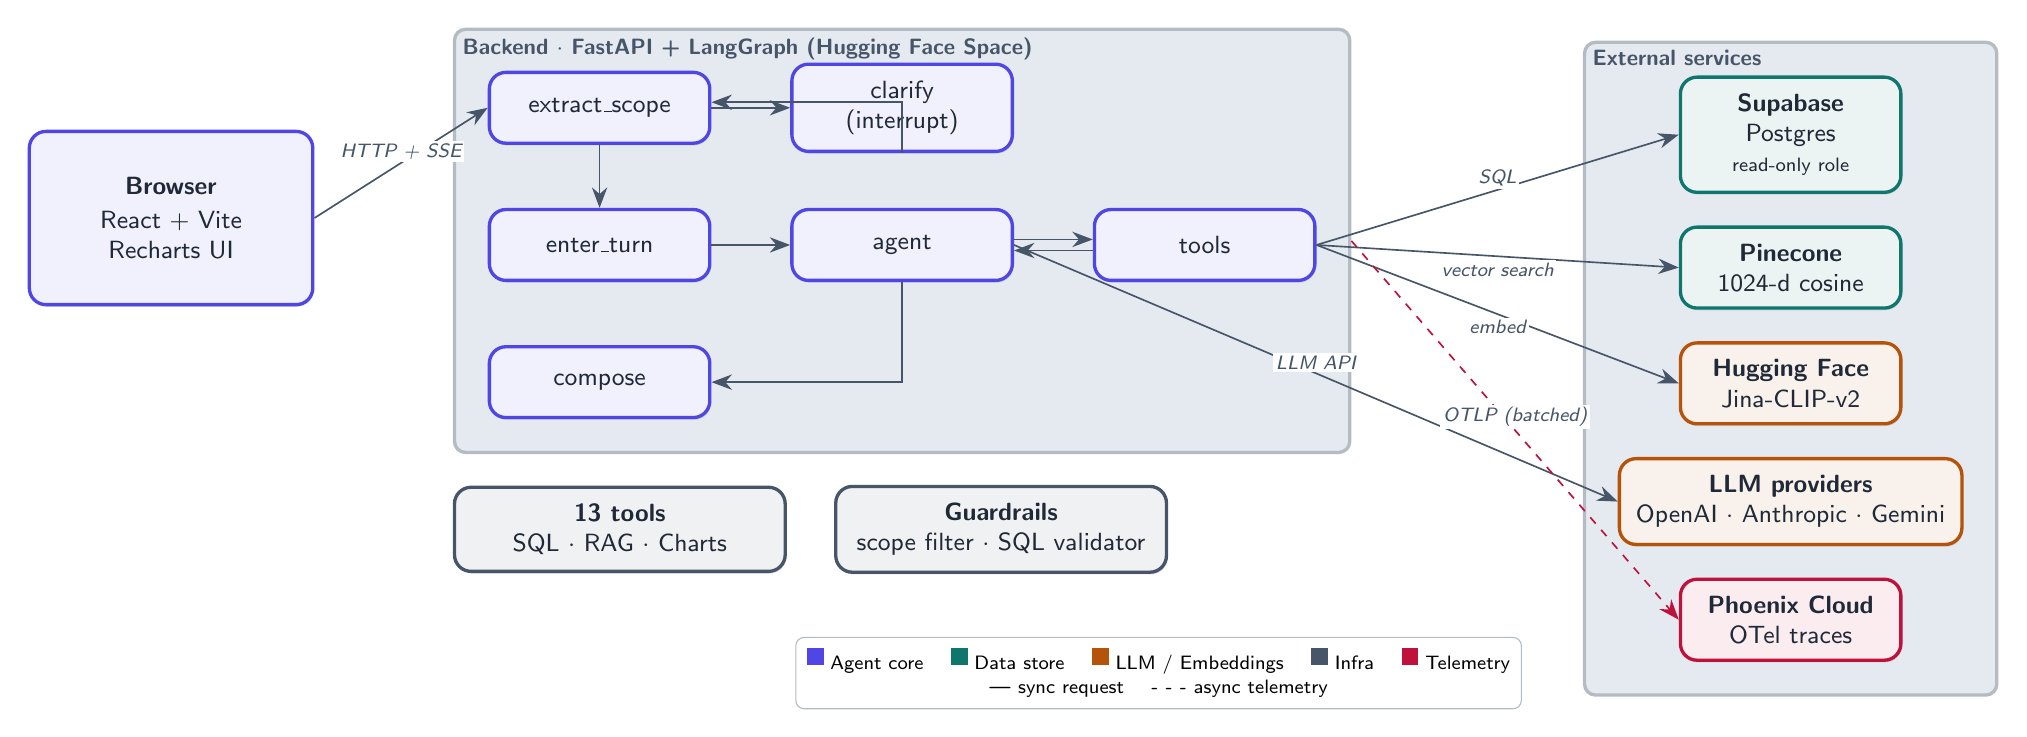
\begin{tikzpicture}[
  font=\sffamily\small,
  node distance=8mm and 8mm,
  every node/.style={align=center},
  lane/.style={rectangle, rounded corners=4pt, draw=slate!40, very thick, fill=slateSoft, inner sep=12pt},
  laneLabel/.style={font=\sffamily\bfseries\footnotesize, slate},
  box/.style={rectangle, rounded corners=6pt, draw=#1, very thick, fill=#1!8, text=ink, inner sep=6pt, minimum height=9mm, drop shadow={shadow xshift=0.4pt, shadow yshift=-0.8pt, opacity=0.25}},
  agentBox/.style={box=indigo, minimum width=28mm},
  dataBox/.style={box=teal, minimum width=28mm},
  llmBox/.style={box=amber, minimum width=28mm},
  obsBox/.style={box=rose, minimum width=28mm},
  infraBox/.style={box=slate, minimum width=28mm},
  arrow/.style={-{Stealth[length=2.6mm]}, semithick, slate},
  dashArrow/.style={-{Stealth[length=2.6mm]}, dashed, semithick, rose},
  edgeLabel/.style={font=\sffamily\scriptsize\itshape, fill=white, inner sep=1pt, text=slate},
]

% ------------------- Client lane (left) -------------------
\node[box=indigo, minimum width=36mm, minimum height=22mm] (browser) {
  \textbf{Browser}\\[1pt]
  React + Vite\\Recharts UI
};

% ------------------- Backend lane (centre) ----------------
% LangGraph mini state machine inside the backend
\node[agentBox, right=22mm of browser, yshift=14mm] (extract) {extract\_scope};
\node[agentBox, right=10mm of extract] (clarify) {clarify\\(interrupt)};
\node[agentBox, below=8mm of extract] (enter) {enter\_turn};
\node[agentBox, right=10mm of enter] (agent) {agent};
\node[agentBox, right=10mm of agent] (toolsN) {tools};
\node[agentBox, below=8mm of enter] (compose) {compose};

% Arrows inside the state machine
\draw[arrow] (extract) -- (clarify);
\draw[arrow] (clarify.south) |- ([yshift=2pt]extract.east);
\draw[arrow] (extract) -- (enter);
\draw[arrow] (enter) -- (agent);
\draw[arrow] ([yshift=2pt]agent.east) -- ([yshift=2pt]toolsN.west);
\draw[arrow] ([yshift=-2pt]toolsN.west) -- ([yshift=-2pt]agent.east);
\draw[arrow] (agent.south) |- (compose.east);

% Group the state machine into a labelled lane
\begin{pgfonlayer}{background}
  \node[lane, fit=(extract)(clarify)(enter)(agent)(toolsN)(compose),
        label={[laneLabel, anchor=north west]north west:Backend $\cdot$ FastAPI + LangGraph (Hugging Face Space)}] (backend) {};
\end{pgfonlayer}

% Tools & guardrails as side-cards under the backend
\node[infraBox, below=4mm of backend.south west, anchor=north west, minimum width=42mm]
  (toolsCard) {\textbf{13 tools}\\SQL $\cdot$ RAG $\cdot$ Charts};
\node[infraBox, right=6mm of toolsCard, minimum width=42mm]
  (guardCard) {\textbf{Guardrails}\\scope filter $\cdot$ SQL validator};

% Browser to backend (SSE)
\draw[arrow] (browser.east) -- node[edgeLabel, above]{HTTP + SSE} (extract.west);

% ------------------- External services lane (right) -------
\node[dataBox, right=46mm of toolsN, yshift=14mm] (postgres) {\textbf{Supabase}\\Postgres\\\scriptsize read-only role};
\node[dataBox, below=4mm of postgres] (pinecone) {\textbf{Pinecone}\\1024-d cosine};
\node[llmBox,  below=4mm of pinecone] (hf) {\textbf{Hugging Face}\\Jina-CLIP-v2};
\node[llmBox,  below=4mm of hf] (llm) {\textbf{LLM providers}\\OpenAI $\cdot$ Anthropic $\cdot$ Gemini};
\node[obsBox,  below=4mm of llm] (phoenix) {\textbf{Phoenix Cloud}\\OTel traces};

\begin{pgfonlayer}{background}
  \node[lane, fit=(postgres)(pinecone)(hf)(llm)(phoenix),
        label={[laneLabel, anchor=north west]north west:External services}] (ext) {};
\end{pgfonlayer}

% Arrows from tools to external services
\draw[arrow] (toolsN.east) -- node[edgeLabel, above]{SQL} (postgres.west);
\draw[arrow] (toolsN.east) -- node[edgeLabel, below=1pt]{vector search} (pinecone.west);
\draw[arrow] (toolsN.east) -- node[edgeLabel, below=1pt]{embed} (hf.west);
\draw[arrow] (agent.east)  -- node[edgeLabel, above]{LLM API} (llm.west);
\draw[dashArrow] (backend.east) -- node[edgeLabel, above]{OTLP (batched)} (phoenix.west);

% Legend
\node[draw=slate!40, rounded corners=3pt, fill=white, inner sep=4pt, font=\sffamily\scriptsize,
      below=8mm of guardCard.south, anchor=north, xshift=20mm] (legend) {
  \textcolor{indigo}{\rule[0.5mm]{6pt}{6pt}}~Agent core \quad
  \textcolor{teal}{\rule[0.5mm]{6pt}{6pt}}~Data store \quad
  \textcolor{amber}{\rule[0.5mm]{6pt}{6pt}}~LLM / Embeddings \quad
  \textcolor{slate}{\rule[0.5mm]{6pt}{6pt}}~Infra \quad
  \textcolor{rose}{\rule[0.5mm]{6pt}{6pt}}~Telemetry \\[1pt]
  \textbf{---}~sync request \quad \textbf{- - -}~async telemetry
};

\end{tikzpicture}}
\caption{System architecture. The LangGraph state machine sits inside the FastAPI backend
on a Hugging Face Space; structured queries hit Supabase Postgres through a read-only
role, vector search hits Pinecone, embeddings are computed by calling the HF-hosted
Jina-CLIP-v2 model, and traces are exported asynchronously to Phoenix Cloud over OTLP.}
\label{fig:arch}
\end{figure}

\subsection{Key design decisions}

\begin{designbox}
\textbf{LangGraph over plain ReAct.} The clarification UX needs a first-class pause /
resume primitive, and conversations need a checkpointer. \texttt{interrupt()} +
\texttt{InMemorySaver} give us both for free; rolling them by hand on top of a raw LLM
loop is busywork that bugs out at edge cases.
\end{designbox}

\begin{designbox}
\textbf{Scope as a first-class graph concept.} Every tool call carries the resolved
\texttt{property\_code}; the tool wrappers in \texttt{guardrails/scope.py} reject any call
without one. The agent literally cannot answer about a different property by accident.
\end{designbox}

\begin{designbox}
\textbf{Read-only Postgres role + allowlist SQL validator.} Even if the LLM emits
malicious or wrong SQL through \texttt{execute\_scoped\_sql}, the
\texttt{property\_reader} role lacks \texttt{INSERT/UPDATE/DELETE/DDL}, and
\texttt{guardrails/sql\_validator.py} rejects multi-statement queries and any statement
that omits a \texttt{property\_code} predicate before it reaches the connection.
\end{designbox}

\begin{designbox}
\textbf{Trusted UI from structured intent.} The LLM emits \texttt{components[]} entries
declaring what it wants to show (e.g.\ ``a line chart of mean rent for these 12 months'');
the backend supplies the actual data from SQL tools, and the frontend renders fixed React
components. The user never sees raw JSON the LLM made up.
\end{designbox}

\begin{designbox}
\textbf{HF-hosted Jina-CLIP-v2 embeddings.} Multimodal (text + image share a 1024-d
space), so a query like ``photo of the pool'' can match a scraped image. Hosting the
weights on Hugging Face instead of bundling them into the backend image keeps the HF
Space slim and cold-start friendly, at the cost of one extra network hop per embedding.
\end{designbox}

\begin{designbox}
\textbf{Chroma $\rightarrow$ Pinecone migration.} V1 used local Chroma --- zero config,
perfect for offline iteration. V2 moved to Pinecone for production: managed, no disk
persistence to babysit on HF Spaces, and the free tier covers our workload. The retrieval
API surface is identical so the rest of the code did not change.
\end{designbox}

\begin{designbox}
\textbf{Runtime LLM switching.} \texttt{llm\_registry.py} treats provider $\times$ model
as a per-request choice. Useful both for cost / quality comparisons and for falling back
when one provider is degraded.
\end{designbox}

\begin{designbox}
\textbf{Typed SSE event protocol.} A single SSE stream carries discriminated events
(\texttt{step}, \texttt{tool}, \texttt{tool\_end}, \texttt{delta}, \texttt{clarification},
\texttt{done}, \texttt{error}). The UI shows live tool progress and per-tool durations,
which materially changed perceived latency on multi-tool turns.
\end{designbox}

\begin{designbox}
\textbf{Phoenix + OpenInference.} OTel-native, vendor-agnostic. We instrument the
libraries, not our code, so a future swap to a self-hosted Phoenix or to another OTel
backend is a one-env-var change. Fail-open everywhere --- a missing key never blocks
\texttt{/chat}.
\end{designbox}

\begin{designbox}
\textbf{APScheduler in-process for evals.} The scheduler runs on its own thread pool
(\texttt{max\_workers=1}, \texttt{coalesce=True}, \texttt{max\_instances=1}) inside the
FastAPI process. No separate worker to operate; overlapping ticks can't pile up; eval
runs never touch the request thread pool.
\end{designbox}

% ===========================================================================
\section{Monitoring \& Evaluation}
% ===========================================================================

This section is intentionally short --- monitoring and evals are first-class subsystems
but they share the same weight as any other component in §3.

\subsection{Tracing (Phoenix Cloud)}

OpenInference instruments LangChain so each LangGraph node and tool call becomes a span,
the three LLM SDKs so token counts / latency / prompts are captured, and FastAPI so each
request gets its own root span. Header sanitisation strips
\texttt{Authorization}, \texttt{X-Admin-Token} and cookies before export.
\texttt{BatchSpanProcessor} ships spans on a background thread so the request hot path is
never blocked, and the whole setup is fail-open --- if the key is missing or the network
is down, the API keeps serving.

\begin{figure}[H]
  \centering
  \includegraphics[width=0.9\linewidth]{screenshots/06-phoenix-trace.png}
  \caption{Phoenix trace tree for a single chat turn: \texttt{extract\_scope}, \texttt{agent},
  per-tool spans with arguments and results, and the LLM SDK calls underneath, all
  durations attached.}
  \label{fig:phoenix}
\end{figure}

\subsection{Eval harness}

\texttt{backend/app/evals/golden\_set.yaml} holds curated regression cases ---
\texttt{\{id, property\_code, question, expected\_substrings, expected\_tools\}}.
\texttt{runner.py} runs each one against the \emph{live} graph (so scope resolution,
guardrails and tool selection are all under test), auto-resumes clarification interrupts
up to twice with sensible defaults, and emits a per-case \texttt{eval.case} span into
Phoenix so any regression links straight back to a trace. \texttt{scorer.py} is an
LLM-as-judge: it prefers \texttt{open\_rag\_eval}'s \texttt{TRECEvaluator} when the API
surface is importable, otherwise falls back to a direct OpenAI judge with a strict
0.25-step rubric that defaults to 0.75 when uncertain. Results land in SQLite
(\texttt{eval\_runs}, \texttt{eval\_cases}) plus a JSONL snapshot under
\texttt{backend/evals/results/}. APScheduler reruns on a cron, and the admin API
(\texttt{/evals/golden}, \texttt{/evals/runs}, \texttt{/evals/schedule}) backs the
Monitoring tab in the UI.

\begin{figure}[H]
  \centering
  \begin{minipage}{0.48\linewidth}
    \centering
    \includegraphics[width=\linewidth]{screenshots/04-monitoring-runs.png}
    \caption{Monitoring tab --- run list.}\label{fig:runs}
  \end{minipage}\hfill
  \begin{minipage}{0.48\linewidth}
    \centering
    \includegraphics[width=\linewidth]{screenshots/05-monitoring-run-detail.png}
    \caption{Single run drilled in.}\label{fig:rundetail}
  \end{minipage}
\end{figure}

\subsection{Sample results}

The numbers below come from the most recent run snapshot
(\texttt{backend/evals/results/20260525T050716Z\_\dots.jsonl}). They reflect a real
end-to-end execution against the live graph; this particular run intentionally exercised
a partially ingested sandbox (\texttt{search\_property\_pages} returned empty context),
which is exactly the failure mode the eval is designed to surface --- groundedness drops
to zero while the agent dutifully refuses to fabricate.

\begin{table}[H]
\centering
\small
\caption{Latest scheduled run --- run \texttt{fcc268a7\dots}, 2 cases, judge \texttt{gpt-4o-mini}.}
\label{tab:eval}
\begin{tabular}{@{}lcccc@{}}
\toprule
\textbf{Metric} & \textbf{Mean} & \textbf{Min} & \textbf{Pass count} & \textbf{Mean duration (ms)} \\
\midrule
groundedness        & 0.00 & 0.00 & 2/2 (no errors) & --- \\
hallucination       & 1.00 & 1.00 & --- & --- \\
answer\_relevance   & 0.25 & 0.00 & --- & --- \\
context\_relevance  & 0.00 & 0.00 & --- & --- \\
\midrule
\multicolumn{4}{l}{Mean per-case latency} & 13{,}542 \\
\bottomrule
\end{tabular}
\end{table}

The harness itself is the deliverable here: re-running it against a fully ingested
property restores the scores. The point is that any regression now shows up as a number
in the Monitoring tab and a linked trace in Phoenix, not as a bug report from a user.

% ===========================================================================
\section{Assumptions, Tradeoffs \& Limitations}
% ===========================================================================

\subsection{Assumptions}

\begin{itemize}
  \item Rent-roll Excel schema matches the provided 12-month sample; columns are detected by header name, not by position.
  \item Property codes are short, unique strings (e.g.\ \texttt{115r}), stable across snapshots.
  \item Reviewer has at least one LLM key; the registry filters to configured providers, so a missing one degrades gracefully.
  \item ``Latest month'' means the most recent ingested \texttt{rent\_snapshots.snapshot\_month}, not the calendar month.
  \item Phoenix Cloud is acceptable for telemetry; without \texttt{PHOENIX\_API\_KEY} everything still works, just without traces.
\end{itemize}

\subsection{Tradeoffs}

\begin{tradeoffbox}
\textbf{\texttt{InMemorySaver} checkpointing.} Conversations evaporate when the backend
restarts. Picked for simplicity; swapping to a Postgres saver is a one-line change if
persistence matters.
\end{tradeoffbox}

\begin{tradeoffbox}
\textbf{HF-hosted embedding model.} Keeps the backend image slim and avoids bundling
$\sim$2~GB of weights into the HF Space, at the cost of one network round-trip per
embedding and a Hugging Face dependency on the hot path.
\end{tradeoffbox}

\begin{tradeoffbox}
\textbf{Chroma $\rightarrow$ Pinecone.} Chroma is unbeatable for local iteration (zero
config, file-backed), but persisting it on a free-tier Space is awkward. Pinecone is
managed and free-tier-friendly, at the cost of an additional vendor.
\end{tradeoffbox}

\begin{tradeoffbox}
\textbf{Allowlist SQL validator.} Some legitimate LLM queries get false-rejected by the
scope-predicate check. We accept the small false-reject rate to bound the blast radius
of any malicious or buggy generated SQL.
\end{tradeoffbox}

\begin{tradeoffbox}
\textbf{Single-property default.} The dropdown supports multi-select and a
\texttt{compare\_units} path exists, but the agent is biased toward single-property
answers because that is the dominant use case.
\end{tradeoffbox}

\begin{tradeoffbox}
\textbf{SSE over WebSockets.} One-way is enough for chat and SSE survives every reverse
proxy we tested. We give up bidirectional features we don't need.
\end{tradeoffbox}

\begin{tradeoffbox}
\textbf{LLM-as-judge.} Cheap, fast, comparable across runs --- but the judge can
self-collude with same-family models. The strict 0.25-step rubric, the requirement to
list concrete issues, and the default-to-0.75 instruction together push the judge away
from cheap perfection.
\end{tradeoffbox}

\begin{tradeoffbox}
\textbf{APScheduler in-process.} Simpler than a separate worker, but eval runs share the
FastAPI VM. If they ever compete with request traffic, the next step is a dedicated
worker process.
\end{tradeoffbox}

\subsection{Limitations / known gaps}

\begin{itemize}
  \item No auth on \texttt{/chat}; the deployed URL is shared by obscurity. \texttt{ADMIN\_TOKEN} guards \texttt{/admin/*} and \texttt{/evals/*} only.
  \item Golden set is hand-curated and small ($\sim$10 cases) --- broader coverage and adversarial / negative cases are the obvious next step.
  \item RAG quality depends on what was ingested per property; if a property page was never \texttt{POST}ed to \texttt{/admin/ingest}, the agent falls back to SQL and says so.
  \item No per-request LLM cost cap; budgets are enforced upstream by the provider account.
  \item Cold-start latency on HF Spaces --- the first request after idle has to wake the Space, and the multimodal embedding endpoint has its own warm-up.
  \item \texttt{compare\_properties} is currently disabled (commented out) pending a clearer UX for $>$2 properties.
\end{itemize}

% ===========================================================================
\section{Reviewer Pointers}
% ===========================================================================

If you're reading the code, this is the shortest path through it:

\begin{itemize}
  \item \texttt{backend/app/graph/build.py} --- LangGraph topology, state-machine wiring, SSE stream.
  \item \texttt{backend/app/graph/nodes.py} --- node implementations including \texttt{extract\_scope} and \texttt{clarify}.
  \item \texttt{backend/app/tools/sql\_tools.py}, \texttt{rag\_tools.py} --- the 13 bound tools.
  \item \texttt{backend/app/guardrails/scope.py}, \texttt{sql\_validator.py} --- the safety story.
  \item \texttt{backend/app/ingestion/v2/} --- docling extractor, structure-aware chunker, doc-store, Pinecone upsert, HF embedding client.
  \item \texttt{backend/app/observability.py} --- Phoenix / OpenInference wiring.
  \item \texttt{backend/app/evals/runner.py}, \texttt{scorer.py}, \texttt{scheduler.py}, \texttt{api.py}, \texttt{golden\_set.yaml}.
  \item \texttt{frontend/src/components/Monitoring.jsx} --- eval admin UI.
  \item \texttt{frontend/src/components/ComponentRenderer.jsx} --- \texttt{components[]} dispatch into KPI cards / charts / tables.
\end{itemize}

\end{document}
